\documentclass[12pt]{article}
\usepackage[english]{babel}
\usepackage{float}
\usepackage[margin=1in]{geometry}
\usepackage{graphicx}
%\usepackage[toc,page]{appendix}
\graphicspath{ {./doc/img/} }
\newcommand{\rpm}{\raisebox{.2ex}{$\scriptstyle\pm$}} 
\usepackage{listings}
\usepackage{xcolor}
\usepackage{indentfirst}
\usepackage[final]{pdfpages}


\begin{document}

\title{Joe Phaneuf \\ Computer Vision 16-720 Spring 2018 \\ Feb. 03, 2018 }
\date{}
\author{}
\maketitle

\newpage


\stepcounter{section}
\section{Q1}
\subsection{Q1.1}

The filter bank contains four types of filter at different scales. The first two filters (gaussian and log) will respond to circular elements, the former containing peaks and the latter containing valleys.
The next two filter types are derivitive filters, which will respond to vertical and horizontal edges respectively.
Figure \label{fig:test_image} shows a test image for the filters, Figure shows \label{fig:filters} the filters themselves, while Figure \label{fig:filter_responses} shows the filtered images.

\begin{figure}[H]
\centering

\includegraphics[page=1,width=0.4\textwidth]{test}
\caption{Test Image}    
\label{fig:test_image}
\end{figure}   

\begin{figure}[H]
\centering
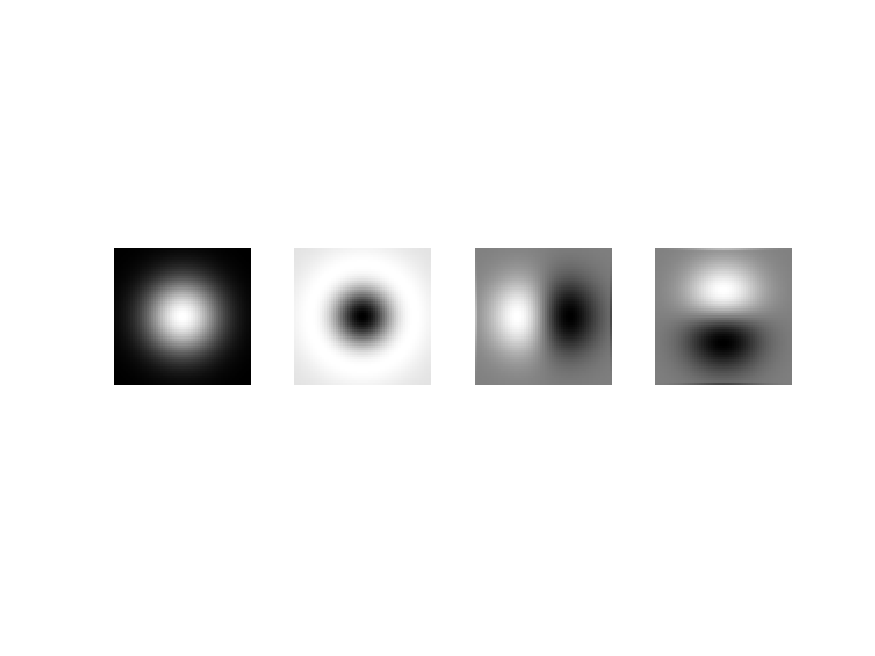
\includegraphics[page=1,width=0.75\textwidth]{q1_filters}
\caption{Filters}    
\label{fig:filters}
\end{figure}   

\begin{figure}[H]
\centering
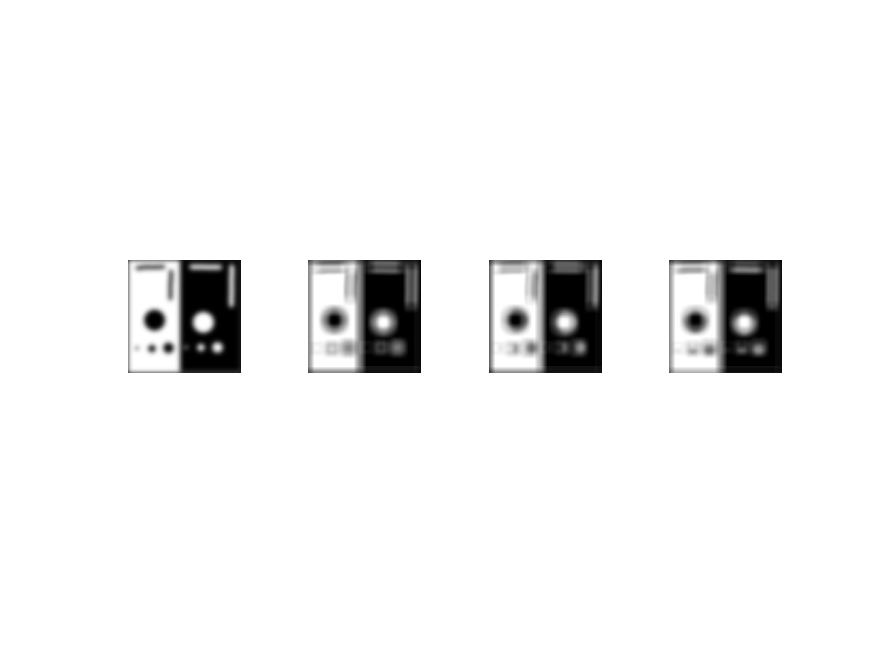
\includegraphics[page=1,width=0.75\textwidth]{q1_responses}
\caption{Filter Responses}    
\label{fig:filter_responses}
\end{figure}   

\newpage
\subsection{Q1.2}

\end{document}



